% !Mode:: "TeX:UTF-8"
\documentclass{article}
% !Mode:: "TeX:UTF-8"
\usepackage[english]{babel}
\usepackage[UTF8]{ctex}
\usepackage{amsmath, amsthm, amssymb}

% Figure
\usepackage{graphicx}
\usepackage{float} %% H can fix the location
\usepackage{caption}
\usepackage[format=hang,singlelinecheck=0,font={sf,small},labelfont=bf]{subfig}
\usepackage[noabbrev]{cleveref}
\captionsetup[subfigure]{subrefformat=simple,labelformat=simple,listofformat=subsimple}
\renewcommand\thesubfigure{(\alph{subfigure})}

\usepackage{epstopdf} %% convert eps to pdf
\DeclareGraphicsExtensions{.eps,.mps,.pdf,.jpg,.png} %% bmp, gif not supported
\DeclareGraphicsRule{*}{eps}{*}{}
\graphicspath{{img/}{figure/}{../figure/}} %% fig directorys

%% \usepackage{pstricks} %% a set of macros that allow the inclusion of PostScript drawings directly inside TeX or LaTeX code
%% \usepackage{wrapfig} %% Wrapping text around figures

% Table
\usepackage{booktabs} %% allow the use of \toprule, \midrule, and \bottomrule
\usepackage{tabularx}
\usepackage{multirow}
\usepackage{colortbl}
\usepackage{longtable}
\usepackage{supertabular}

\usepackage[colorinlistoftodos]{todonotes}

% Geometry
\usepackage[paper=a4paper, top=1.5cm, bottom=1.5cm, left=1cm, right=1cm]{geometry}
%% \usepackage[paper=a4paper, top=2.54cm, bottom=2.54cm, left=3.18cm, right=3.18cm]{geometry} %% ms word
%% \usepackage[top=0.1cm, bottom=0.1cm, left=0.1cm, right=0.1cm, paperwidth=9cm, paperheight=11.7cm]{geometry} %% kindle

% Code
%% \usepackage{alltt} %% \textbf can be used in alltt, but not in verbatim

\usepackage{listings}
\lstset{
    backgroundcolor=\color{white},
    columns=flexible,
    breakatwhitespace=false,
    breaklines=true,
    captionpos=tt,
    frame=single, %% Frame: show a box around, possible values are: none|leftline|topline|bottomline|lines|single|shadowbox
    numbers=left, %% possible values are: left, right, none
    numbersep=5pt,
    showspaces=false,
    showstringspaces=false,
    showtabs=false,
    stepnumber=1, %% interval of lines to display the line number
    rulecolor=\color{black},
    tabsize=2,
    texcl=true,
    title=\lstname,
    escapeinside={\%*}{*)},
    extendedchars=false,
    mathescape=true,
    xleftmargin=3em,
    xrightmargin=3em,
    numberstyle=\color{gray},
    keywordstyle=\color{blue},
    commentstyle=\color{green},
    stringstyle=\color{red},
}

% Reference
%% \bibliographystyle{plain} % reference style

% Color
\usepackage[colorlinks, linkcolor=blue, anchorcolor=red, citecolor=green, CJKbookmarks=true]{hyperref}
\usepackage{color}
\def\red#1{\textcolor[rgb]{1.00,0.00,0.00}{#1}}
\newcommand\warning[1]{\red{#1}}

% Other
%% \usepackage{fixltx2e} %% for use of \textsubscript
%% \usepackage{dirtree}  %% directory structure, like the result of command tree in bash shell


% !Mode:: "TeX:UTF-8"
%+++++++++++++++++++++++++++++++++++article+++++++++++++++++++++++++++++++++
%customize the numbering of equation, to make it like section-subsection-equation style, for example,1-2-3
\makeatletter\@addtoreset{equation}{subsection}\makeatother
\renewcommand\theequation{%
\thepart\arabic{section}%
-\thepart\arabic{subsection}%
-\thepart\arabic{equation}%
}
%theorem
\newtheorem{definition}{D\'efintion} %% 整篇文章的全局编号
\newtheorem*{thmwn}{Thm} %% without numbers
\newtheorem{theorem}{Th\'eor\`eme}[section] %% 从属于section编号
\newtheorem{corollary}{Corollary}[theorem] %% 从属于theorem编号
\newtheorem{lemma}{Lemma}
\newtheorem{proposition}{Proposition}[section]
\newtheorem{example}{Example}
\newtheorem*{attention}{Attention}
\newtheorem*{note}{Note}
\newtheorem*{remark}{Remark}
\newtheorem{question}{Question}[section]
\newtheorem{problem}{Problem}
\newtheorem{fact}{Fact}


\begin{document}
\title{Programming Paradigms\\ Eric's notes}
\author{Eric Wang}
\maketitle
\newpage
\tableofcontents
\newpage
\section{Lecture 1 - 基本介绍}
C procedure paradigm\\
Assembly 汇编\\
C++\\
Concurrent Programming 并发编程\\
Sequential Programming 顺序

Scheme Lisp functional paradigm\\
You always rely on the return value of a function to move forward, And you program without side effects

Python

\section{Lecture 2}
The memory system as a whole is organized as a large array of bytes. Every byte has its
own "address" which is like its index in the array.

The byte is sometimes defined as the "smallest addressable unit" of memory. Most computers also support reading and writing larger units of memory— 2 byte "half-words" (sometimes known as a "short" word) and 4 byte "words".

Half-words and words span consecutive bytes in memory. By convention the address of any multiple-byte thing is the address of its lowest byte— its "base-address".

Most computers restrict \textbf{half-word} and word accesses to be "aligned"—
\indent a \textbf{half-word} must \textbf{start at an even address} and \\
\indent a \textbf{word} must \textbf{start} at an \textbf{address that is a multiple of $4$}.

The ASCII code defines $128$ characters and a mapping of those characters onto the numbers $0..127$.

All standard ASCII characters have \textbf{zero in the uppermost bit (the "most significant" bit)} since they only span the range $0..127$.

\subsection{不同数据类型间的赋值}
\begin{verbatim}
low-level memory
C/C++
bool
char            1 byte
short           2 bytes
int             4 bytes
long            4 bytes
float           4 bytes
double        	8 bytes
binary digit => bit
Byte=> 8 bits   2^8=256
\end{verbatim}
Currently almost all machines use $4$ bytes to store an address, creating a $4$GB addressable range.\\
Because each byte of memory has to have an address. In a $32$-bit operating system, an address is $32$ bits long; thus, there are $2^{32}$ possible addresses, which means there are $2^{32}$ bytes $= 4$ GB.

Some processors have a special hardware Floating Point Unit, FPU, that substantially speeds up floating point operations.

Instruction— Machine instructions themselves are also encoded using bit patterns,most often using the same 4-byte native word size. The different bits in the instruction encoding indicate things such as what type of instruction it is (load,store, multiply, etc.) and the registers involved.

\subsection{负数的表示}
\begin{verbatim}
0111,1111,1111,1111
\end{verbatim}
如果最左端的$0$是一个$1$, 那么这个$1$ 会贡献$2^{15}$, 当上面的数字加上$1$ 之后, 刚好变成了$1000,0000,0000,0000$\\
所以原来的那个数是$2^{15} – 1$

\textbf{正负整数}\\
第一位$0$表示正, $1$表示负, $(-1)^0=1, (-1)^1 = -1$
\begin{verbatim}
7: 0000,0000,0000,0111
\end{verbatim}
我们最开始想到的 $-7$ 的表示方法,就是把第一位$0$变成$1$
\begin{verbatim}
-7:1000,0000,0000,0111
\end{verbatim}

我们希望计算机硬件能够尽量简单优雅的进行加法和减法
\begin{verbatim}
7 + (-7) = 0
7: 0000,0000,0000,0111
-7:1000,0000,0000,0111
1000,0000,0000,1110  相加的结果不等于0, 所以这样表示负数是不行的

0: 0000,0000,0000,0000
让所有位上的数字全部变成0, 但是让他们都变成1 更加简单
0000,0000,0000,1111  //15
1111,1111,1111,0000
1111,1111,1111,1111 //相加后全部变成了1
\end{verbatim}
对于short而言, 1111,1111,1111,1111 就差$1$ 被清零, 因为加上$1$ 之后, 由于进位导致出现了9个bits, 但是short类型只有8 个bits(overflow), 所以最高位的1 被忽略掉, 所以
\begin{verbatim}
1111,1111,1111,1111 + 1 = 0
\end{verbatim}
我们发现
\begin{verbatim}
0000,0000,0000,1111  //15
1111,1111,1111,0000
\end{verbatim}
这两个数的和 然后再加上1 就是0, 所以如果我们将1111,1111,1111,0000加上1 刚好就是 -15, 也就是说
\begin{verbatim}
-15: 1111,1111,1111,0001
\end{verbatim}
所以得到一个正数的相反数, 就是将这个正数的所有二进制取反(补码), 然后再加上1

\section{Lecture 3}
\begin{table}[htbp]
\caption{int intArray[6]}
  \centering
\begin{tabular}{|c|c|c|c|c|c|}
\hline
  intArray[0] & intArray[1] & intArray[2] & intArray[3] & intArray[4] & intArray[5] \\
\hline
\end{tabular}
\end{table}
\begin{verbatim}
int array[10]
array \equiv &array[0]
array + k \equiv &array[k]
\end{verbatim}

\verb+void swap(int *a, int *b)+

\section{Lecture 4}
\subsection{Arithmetic on a void pointer}
For a \verb (void*) pointer, array subscripting and pointer arithmetic don't quite make sense.
These manipulations include implicit multiplication by the size of the element type, and
what is sizeof(void)?  Unknown!

有些编译器将size(void) 设为1, 和 char *的大小一样, 但是如果我们利用这个特性, 那我们的code 将不具有可移植性, 所以要明确的进行转换

\begin{lstlisting}[language = C]
void *ptr;
p = (char*)ptr + 4;  // increments ptr by exactly 4, no extra multiplication
\end{lstlisting}
Note that you do not need to cast the result back to (void*), a (void*) is the "universal
recipient" of pointer types and can be freely assigned any type of pointer.  It is best to
use casts only when you absolutely must.

\subsection{函数通过void 指针的通用化}
\begin{lstlisting}[language = C]
void swap(int *a, int *b){
int temp=*a;
*a= *b;
*b= temp;
}
\end{lstlisting}
能够只交换指针吗?

generic version: size 表示需要提取多少个字节来表示数据
\begin{lstlisting}[language = C]
void swap(void *a, void *b, int size){
char buffer[size];
memcpy(buffer, a, size);
memcpy(a, b, size);
memcpy(b, buffer, size);
}
\end{lstlisting}
在使用的时候, 要注意a与b的类型要一致
\begin{lstlisting}[language = C]
int i=44;      	short s=5;
swap(&i, &s, sizeof(short)); //error
swap(&i, &((int)s), sizeof(int)); // does it work?
char *husband = strdup("Fred");
char *wife = strdup("Willma");
swap(&husband, &wife, sizeof(char *));
swap(husband, wife, sizeof(char *)); //error
\end{lstlisting}
交换了4个字节的内容, 指针的长度都是4 个字节

\begin{lstlisting}[language = C]
void * lsearch(void* key, void * base, int n, int elemSize){
// n base 数列中有多少个值, elemSize 元素的字节数
for (int i=0; i<n; i++){
void * elemAddr = (char *)base + i * elemSize;	
//void * elemAddr = base + i * elemSize; error 不同类型的数据指针加1 的偏移量不一样
if(memcmp(key, elemAddr, elemSize) == 0)
	return elemAddr;
}
return null;
}

void * lsearch(void *key, void *base, int n, int elemSize, int (* cmpfun)(void *, void *))
// cmpfun 用户提供的比较函数
\end{lstlisting}

\section{Lecture 5}
\begin{lstlisting}[language = C]
void * lsearch(void *key, void *base, int n, int elemSize, int (* cmpfun)(void *, void *)){
for (int i=0; i<n; i++){
void * elemAddr = (char *)base + i * elemSize;	
if(cmpfun(key, elemAddr) == 0)
	return elemAddr;
}
return null;
}
\end{lstlisting}
For example:
\begin{lstlisting}[language = C]
int array[]={4, 2, 3, 7, 11, 6};
int number=7;
int *found=lsearch(&number, array, 6, sizeof(int), intcmp);
int intcmp(void *elem1, void *elem2){
int *ip1 = (int *)elem1;
int *ip2 = (int *)elem2;
return *ip1 - *ip2; // 最好是返回-1, 0, 1, 因为相减可能overflow
}

char *notes[] = {"Ab", "F#", "B", "Gb", "D"}; //每个元素都是一个字符数组
char *favoriteNote = "Eb";
char ** found = lsearch(&favoriteNote, notes, 5, sizeof(char *), StrCmp);
notes 是 char ** 类型的

int StrCmp(void *vp1, void *vp2){
char * s1 =  *(char **)vp1; // (char *)vp1 error
char * s2 =  *(char **)vp2;
return strcmp(s1, s2);
}

// 下面的方法也可以, 但是不推荐, 你要清楚的知道你在做什么!!!
char ** found = lsearch(favoriteNote, notes, 5, sizeof(char *), StrCmp);
int StrCmp(void *vp1, void *vp2){
char * s1 =  (char *)vp1;
char * s2 =  *(char **)vp2;
return strcmp(s1, s2);
}

void * bsearch(void *key, void *base, int n, int elemsize, int (* cmp)(void *, void *))
\end{lstlisting}

function and method 是不同的

method 是与object相关的, 含有隐含的this 指针

\subsection{C 中模仿类实现stack}
\textbf{stack.h}
\begin{lstlisting}[language = C]
// a stack data structure
typedef struct {
int *elems;
int logicalLen;
int allocLen;
} stack;
// 这里我们要存储的元素是int类型的, 我们定义的栈结构中int *elems, 所以我们实际上在栈中存储的是我们想要存储东西的指针, 在这里, 也就是说栈中的元素是int *类型的

void stackNew(stack *s);  // 模仿类的初始化函数
void stackDispose(stack *s);  //模仿类的析构函数
void stackPush(stack *s, int value);  // 检测边界, 需要重新申请空间然后复制元素后再添加
int stackPop(stack *s);
\end{lstlisting}

\textbf{stack.c}
\begin{lstlisting}[language = C]
void stackNew(stack *s){
s->logicalLen = 0;
s->allocLen = 4;
s->elems = (int *)malloc(4*sizeof(int));
assert(s->elems !=NULL); // 检查申请空间成功与否
}
\end{lstlisting}

\section{Lecture 6}
\begin{lstlisting}[language = C]
void stackDispose(stack *s){
free(s->elems);
}
// 我们不需要free(s) , s可能是一个局部变量, 我们只需要释放我们申请的空间

void stackPush(stack *s, int value){
if(s->logicalLen == s->allocLen){
	s->allocLen *= 2;
	s->elems = realloc(s->elems, s->allcLen * sizeof(int));
	assert(s->elems != NULL);
}
s->elems[s->logicalLen] = value;
s->logicalLen ++;
}
// realloc 对malloc申请的内存进行动态调整, 同时它会自动对原来的空间进行处理, 所以不需要我们手动处理

int stackPop(stack *s){
assert(s->logicalLen > 0);
s->logicalLen --;
return s->elems[s->logicalLen];
}
\end{lstlisting}

\subsection{C 中模仿类实现stackd的泛型化}
\textbf{stack.h}
\begin{lstlisting}[language = C]
typedef struct{
void *elems;
int elemsize;
int logicalLen;
int allocLen;
}stack;
// 这里我们要存储的元素是void类型的, 我们定义的栈结构中void *elems, 所以我们实际上在栈中存储的是我们想要存储东西的指针, 在这里, 也就是说栈中的元素是void *类型的

void stackNew(stack *s, int elemsize);
void stackDispose(stack *s);
void stackPush(stack *s, void *elemAddr); //elemAddr要存储的元素的地址
void stackPop(stack *s, void *elemAddr); //出栈元素放到elemAddr地址中
\end{lstlisting}

\textbf{stack.c}
\begin{lstlisting}[language = C]
void stackNew(stack *s, int elemsize){
s->elemsize = elemsize;
s->logicalLen = 0;
s->allocLen = 4;
s-> elems = malloc(4 * elemsize);
assert(s->elems != NULL);
}

void stackDispose(stack *s){
free(s->elems);
}

static void stackGrow(stack *s){
s->allocLen *= 2;
s->elems = realloc(s->elems, s->allocLen * elemsize);
}
//static 这个函数只能在本文件中使用,

void stackPush(stack *s, void *elemAddr){
if (s->logicLen == s->allocLen)
	stackGrow(s);
void *target = (char *)s->elems + s->logicalLen * s->elemsize;
memcpy(target, elemAddr, s->elemsize);
s->logicalLen ++;
}

void stackPop(stack *s, void *elemAddr){
s->logicalLen --;
void *source = (char *)s->elems + s->logicalLen * s->elemsize;
memcpy(elemAddr, source, s->elemsize);
}
//我们也可以void * stackPop(stack *s), 但是这样需要在函数中动态申请内存, 这样代码会变得很难维护, 所以不推荐那样做
\end{lstlisting}

\section{Lecture 7}
\subsection{内存释放}
\begin{lstlisting}[language = C]
int main(){
const char *friends[] = {"AI", "Bob", "Eric"};
stack stringstack;
stackNew(&stringstack, sizeof(char *));
for (int i=0; i<3; i++){
	char *copy = strdup(friends[i]);
	stackPush(&stringstack, &copy);
}
\end{lstlisting}
\textbf{strdup会调用malloc, 所以之后我们需要将其释放掉}

这里我们要存储的元素是char *类型的, 我们定义的栈结构中void *elems, 所以我们实际上在栈中存储的是我们想要存储东西的指针, 在这里, 也就是说栈中的元素是char **类型的

\begin{lstlisting}[language = C]
char *name;
for (int i=0; i<3; i++){
	stackPop(&stringstack, &name);
	printf("%s",name);
	free(name);
}
stackDispose(&stringstack);
}

void stackNew(stack *s, int elemsize, void (* freefun)(void *))
//freefun 是释放栈中元素空间的函数, 需要用户提供, 因为我们不知道元素是指针还是普通元素

typedef struct{
void *elems;
int elemsize;
int logicalLen;
int allocLen;
void *freefun;
}stack;


void stackDispose(stack *s){
if(s->freefun !=NULL){
	for(int i=0; i< s->logicLen; i++){
		s->freefun((char *)s->elems + i * s->elemsize);
}
}
free(s->elems);
}

stack stringstack;
stackNew(&stringstack, sizeof(char *), stringFree);

void stringFree(void *elem){
	free(*(char **)elem);
}
\end{lstlisting}
如果我们存储的是int 等类型, 我们只需要将freefun 传入NULL

\bigskip\noindent
\textbf{memcpy 拷贝的两个地址区域不能overlap, memcpy不会进行检查, 所以可能会出错\\
memmove 会检查重叠的区域, 但是执行效率要比memcpy低}

\begin{figure}[htbp]
	\centering
	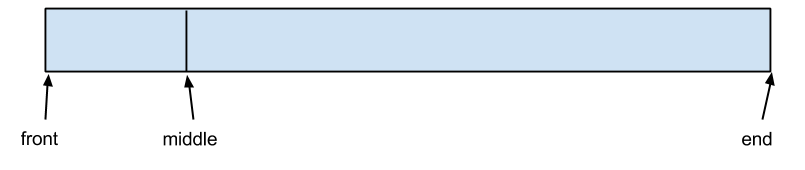
\includegraphics[scale = 0.4]{rotate}\\
	\caption{编程范式 rotate}\label{fig.rotate}
\end{figure}

将middle与end之间的移动到前面, 同时将front与middle之间的移动到后面
\begin{lstlisting}[language = C]
void rotate(void *front, void *middle, void *end){
int frontSize = (char *)middle - (char *)front;
int backSize = (char *)end - (char *)middle;
char buffer[frontSize];
memcpy(buffer, front, frontSize);
memmove(front, middle, backSize);
memcpy((char *)end - frontSize, buffer, frontSize);
}

void qsort(void *base, int n, int elemSize, int (*cmpfn)(void *, void *))
\end{lstlisting}

\section{Lecture 8}
\subsection{malloc, realloc, free}
\begin{figure}[htbp]
	\centering
	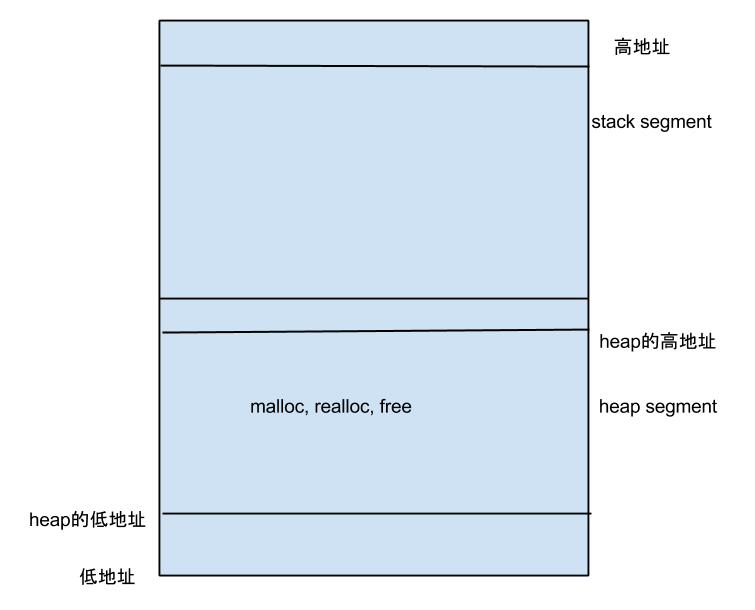
\includegraphics[scale = 0.4]{memo_segment}\\
	\caption{内存分段}\label{fig.memo.segment}
\end{figure}

\begin{lstlisting}[language = C]
foo(){
int a;
int b;
}
\end{lstlisting}
读到a的时候, 将a 压入内存中的stack区域
\begin{figure}[htbp]
	\centering
	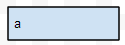
\includegraphics[scale = 0.7]{stack_push-a}\\
	\caption{压a 进入stack之后}\label{fig.stack.push.a}
\end{figure}
然后读到b, 再将b 压入stack中, 由于内存中下方的地址是低地址, 所以是从下方压栈, 所以b在a的下方, 也就是说b在低地址, a在高地址
\begin{figure}[htbp]
	\centering
	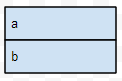
\includegraphics[scale = 0.7]{stack_push-ab}\\
	\caption{压a再压b 进入stack之后}\label{fig.stack.push.ab}
\end{figure}
 \bigskip
\subsubsection{heap segment}
在使用malloc 申请 堆内存的时候
\begin{lstlisting}[language = C]
int *a = malloc(40 * sizeof(int));
\end{lstlisting}
我们不光得到了160个字节的内存,  我们还得到了这160个字节前面的4 个或者8 个字节(具体是4 个还是8 个取决于具体的机器).
\begin{figure}[htbp]
	\centering
	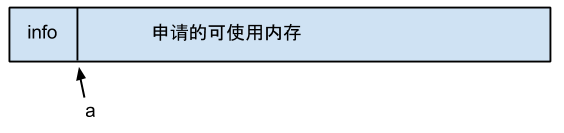
\includegraphics[scale = 0.4]{malloc}\\
	\caption{编程范式 malloc}\label{fig.malloc}
\end{figure}

前面的多出来的额外的字节记录了这个申请到的内存的一些信息, 比如大小等等
这样, 当我们执行free(a) 的时候, 内核会从a 的地址处倒退4 个或者8 个字节, 提取出这个申请的内存的大小信息, 然后将这么大小的内存回收到堆中.
但是当我们执行free(a + 40) 的时候, 内核会将 a+40 这个地址的前4 个或者 8 个字节解释成内存大小信息, 导致error

\bigskip
\textbf{启发式策略}\\
将堆内存划分成不同的区域, 在每个区域中, 当遇到申请内存的请求时, 分配出固定大小的内存, 而不是按照用户传给的数字的精确值, 这样可以更加快速的分配内存
\begin{figure}[htbp]
	\centering
	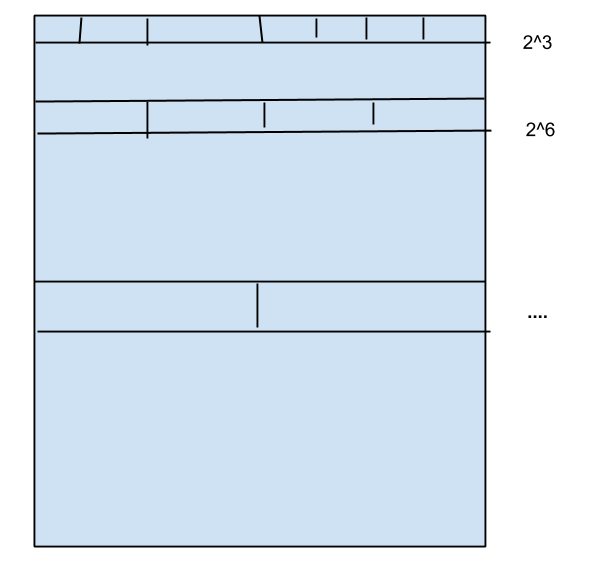
\includegraphics[scale = 0.4]{heuristic-strategies}\\
	\caption{编程范式 启发式策略}\label{fig.heuristic-strategies}
\end{figure}

例如 $malloc(4)$ 发现 $4 < 2^3$, 所以直接在$2^3$ 这个区域分配出$8$ 个子节大小的内存

\textbf{内存压缩}\\
当malloc 遇到一个请求, 但是目前堆中没有连续的内存能够满足这个请求, 但是我们发现未被使用的内存的和是大于这个请求值的.
所以我们可以采用内存压缩的策略, 将用过的内存压缩到一起(内存搬运), 然后就可以继续处理用户的请求
但是这样内存管理就会遇到一个问题, 就是我们必须将已经分配的内存指针$a$ 和 $b$ 更新, 让他们指向新的位置, 否则用户是不知道的
handle
当申请内存的时候, 不返回direct pointer to the data(不是直接指数据的指针), 而是一个距离实际数据有两跳的指针, 也就是说相当于二级指针
\begin{figure}[htbp]
	\centering
	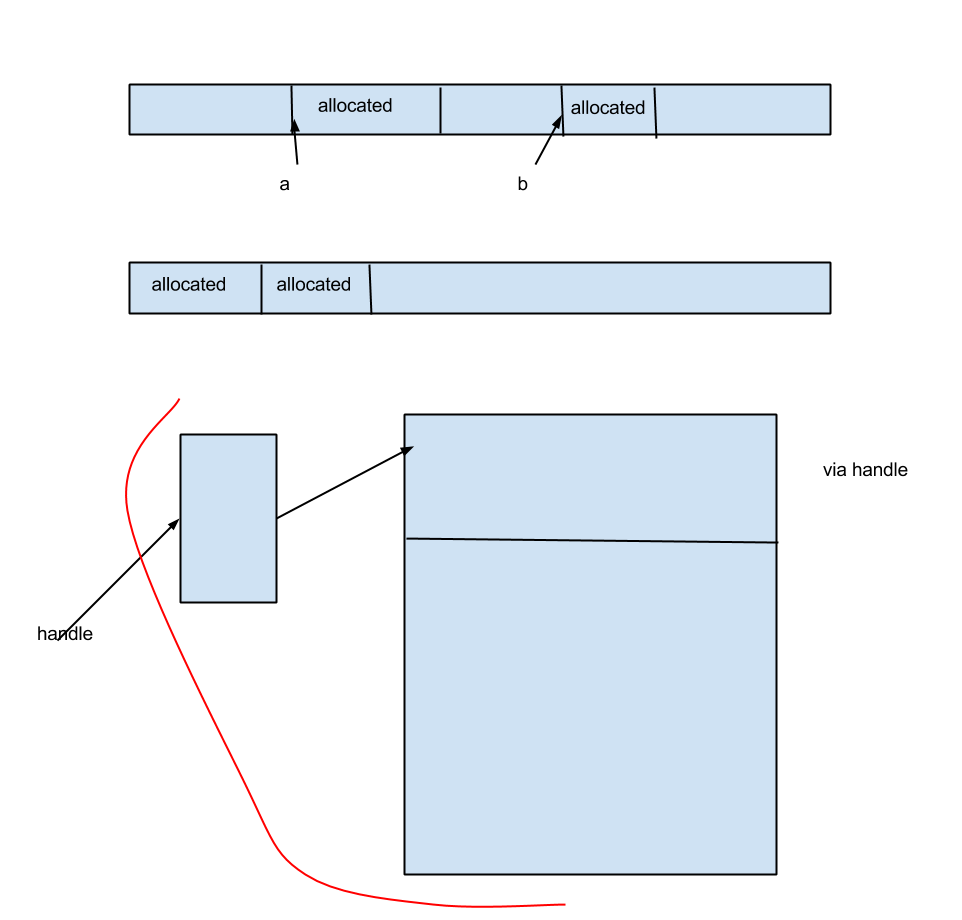
\includegraphics[scale = 0.4]{memo_compression}\\
	\caption{编程范式 内存压缩}\label{fig.memo.compression}
\end{figure}

这样, 当我们进行内存压缩的时候, 只需要对红线右边的进行改动, 对用户的操作则没有影响
但是, 我们必须确保用户对数据的操作与内存压缩这两个操作不能同时发生, 否则会出现问题, 所以需要使用安全锁机制
\begin{lstlisting}[language = C]
void **handle = NewHandle(40);
HandleLock(handle);
... do sth...
HandleUnlock(handle);

\subsubsection{stack segment}
void A(){
int a;
B();
}
\end{lstlisting}
\begin{figure}[htbp]
	\centering
	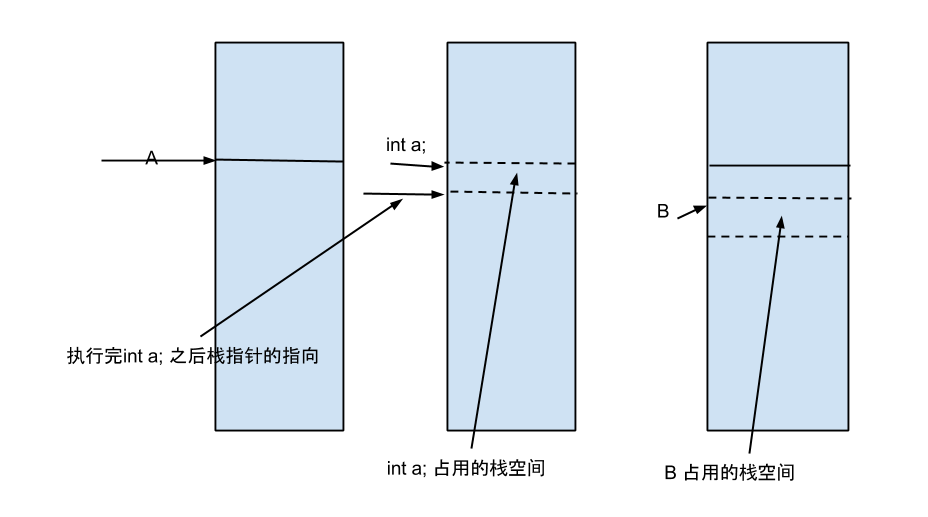
\includegraphics[scale = 0.4]{stack_call}\\
	\caption{编程范式 栈的调用原理}\label{fig.stack.call}
\end{figure}

每次调用一个函数, 栈指针就向下移动(减去刚刚占用的空间), 然后当调用的函数返回时, 栈指针再向上移动, 回到原来的位置

\section{Lecture 9 - 汇编}
在这门课中, 老师invented a assembly language
小型的伪汇编语言
所有的汇编指令都是4字节, 也就是32位宽

\begin{lstlisting}[language = C]
int i;
int j;
i = 10;
j = i + 7;
j ++;

M[R1 + 4] = 10; //store operation

R2 = M[R1+4]; //load operation
R3 = R2 + 7; //ALU operation
M[R1] = R3; //store operation

R2 = M[R1];
R2 = R2 + 1;
M[R1] = R2;
\bigskip\rule{6.8cm}{0.2em}

int i;
short s1;
short s2;
i=200;
s1=i;
s2=s1+1;
\end{lstlisting}
\begin{figure}[htbp]
	\centering
	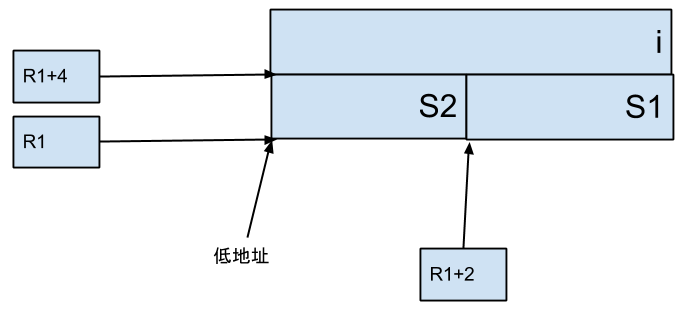
\includegraphics[scale = 0.4]{assembly_short}\\
	\caption{编程范式 汇编 short}\label{fig.assembly.short}
\end{figure}


\begin{lstlisting}[language = C]
M[R1+4]=200;

R2 = M[R1+4];
M[R1+2] = .2 R2  //取出R2的2个字节, 默认的都是.4, 没有写出来
R2=.2 M[R1+2];
R3=R2+1;
M[R1] = .2 R3;
\end{lstlisting}

\subsection{for循环}
\begin{lstlisting}[language = C]
int array[4];
int i;
for (i=0; i<4; i++){
	array[i]=0;
}
\end{lstlisting}
\begin{figure}[htbp]
	\centering
	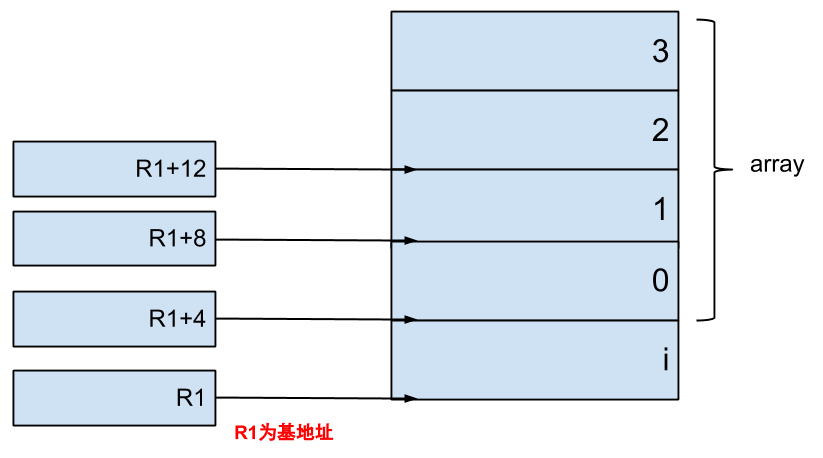
\includegraphics[scale = 0.4]{assembly_array}\\
	\caption{编程范式 汇编 array}\label{fig.assembly.array}
\end{figure}

\begin{lstlisting}[language = C]
M[R1] = 0;

R2 = M[R1]
BEQ R2, 4,  PC+40 //跳转到JMP PC - 40后面的R2=M[R1]
R3=M[R1]
R4=R3*4
R5=R1+4
R6=R4+R5
M[R6] = 0

R2=M[R1]
R2=R2+1
M[R1]=R2
JMP PC - 40 //跳转10条语句

R2=M[R1]
R2=R2-1
M[R1]=R2
\end{lstlisting}
\textbf{汇编代码中, 从上往下是地址从低到高, 所以 PC + 是往下走, PC - 是往上走}

\bigskip\noindent
\textbf{BEQ R2, 4,  PC+40  // 如果 $R2 >=4$ 就跳转到 PC+40}\\
PC 特殊寄存器, 程序计数器, 存储着当前指令的地址\\
BEQ  branch on equal or greater\\
BNE branch on not equal\\
BLT branch on less than\\
BLE branch on less than or equal to\\
BGT branch on greater than\\
BGE branch on greater than or equal to\\

\subsection{operation code操作码}
表示这个机器支持的汇编操作类型,
例如:
\begin{verbatim}
000000	R1=M[R2+4]
000001	R1=1000
010011	R3=R6*R10
111111	M[R1-20]=R19
\end{verbatim}
这里我们采用的是定长编码,
实际上也可以是变长编码,
例如:
\begin{verbatim}
000
001001
\end{verbatim}

\section{Lecture 10} important
函数
\begin{lstlisting}[language = C]
void foo(int bar, int *baz){
char snink[4];
short *why;
}
\end{lstlisting}
\begin{figure}[htbp]
	\centering
	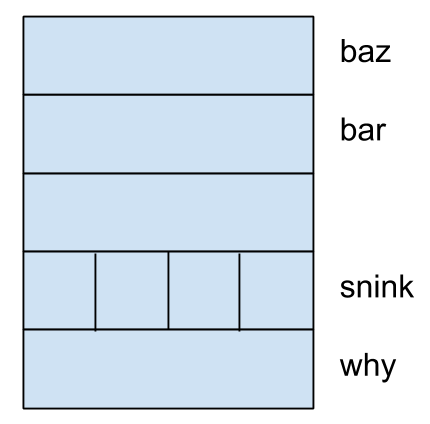
\includegraphics[scale = 0.4]{activation-foo}\\
	\caption{编程范式 activation foo}\label{fig.activation.foo}
\end{figure}


\begin{lstlisting}[language = C]
int main(int argc, char **argv){
int i=4;
foo(i,&i);
return 0;
}
\end{lstlisting}

sp特殊寄存器:
static pointer 指向执行栈的最低地址, 也就是之前我们一直使用的基地址R1

RV 特殊寄存器:
存放函数的返回值

\begin{lstlisting}[language = C]
int fact(int n){
if (n == 0)
	return 1;
return n * fact(n-1);
}
\end{lstlisting}

\section{Lecture 11}
\begin{lstlisting}[language = C]
void foo(){
int x;
int y;
x=11
y=
swap(&x, &y);
}
\end{lstlisting}
\begin{figure}[htbp]
	\centering
	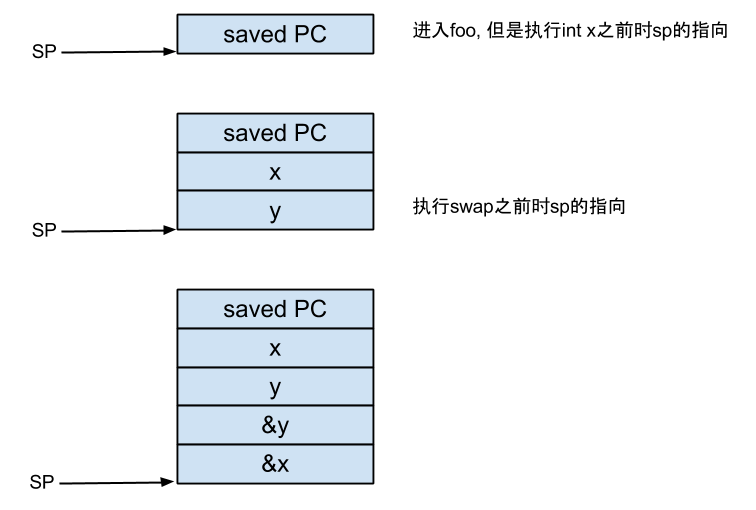
\includegraphics[scale = 0.4]{assembly_fun}\\
	\caption{编程范式 汇编 fun}\label{fig.assembly.fun}
\end{figure}


\begin{lstlisting}[language = C]
void swap(int *x, int *bp){
int temp=*ap;
*ap=*bp;
*bp=temp;
}
SP=SP - 8; //写完这个申请空间的语句, 就立刻补上回收空间的语句,  然后return
M[SP + 4] = 11;
M[SP] = 17;

R1=SP; //\&y
R2=SP+4; //\&x
SP=SP-8;
M[SP] = R2;
M[SP+4] = R1;
CALL <swap>
SP=SP+8;

SP=SP + 8;
RET;		//return
\end{lstlisting}

\begin{figure}[htbp]
	\centering
	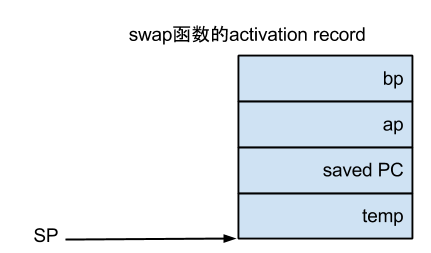
\includegraphics[scale = 0.4]{assembly_swap}\\
	\caption{编程范式 汇编 swap}\label{fig.assembly.swap}
\end{figure}

\begin{lstlisting}[language = C]
<swap>:
SP = SP-4;
//temp=*a
R1=M[SP+8]
R2=M[R1]
M[SP] = R2
//*a=*b
R1=M[SP+12]
R2=M[R1]
R3=M[SP+8]
M[R3] = R2
//*b=temp;
R1=M[SP]
R2=M[SP+12]
M[R2] = R1
SP=SP+4  // 回到进入swap函数时的地址
RET;
\end{lstlisting}

\subsection{C++ reference}
C++中 \& 表示的引用 reference\\
the way references work is that they are basically just automatically dereferenced pointers.\\
所以在将C++ code 编译成汇编代码后, 和C的汇编代码几乎一样\\

引用:就是给变量起一个别名.引用与它所引用的变量共享存储单元
\begin{lstlisting}[language = C]
int i;
int &j=i;  //此时, j 和i 共享一段内存
int k=9
j=k;  //i 的值也为9
j++; // i 的值为10
\end{lstlisting}

引用用作函数参数
\begin{lstlisting}[language = C]
void swap(int &a, int &b){
int temp=a;
a=b;
b=a;
}
i=10; j=20;
swap(i, j); //right
swap(&i, &j);

int x=17;
int y=x;
int &z=y;
int *z=&y;
int *z=y;
\end{lstlisting}

binky是一个C++ class, minky是 class binky的一个method
\begin{lstlisting}[language = C]
binky b;
b.minky(\&n);//这个语句实际上是 binky::minky(\&b, \&n)
\end{lstlisting}
在minky的 activation record, saved PC上面依次是\&n, \&b

static 有76 种意思.

\subsection{preprocessing}
预处理会对
\begin{verbatim}
#define
#include
\end{verbatim}
进行处理

\section{Lecture 12}
\begin{lstlisting}[language = C]
#define 	MAX(a,b)	(((a) > (b)) ? (a) : (b))
MAX(m++, n++) 最终会使较大的值进行2 次自增操作, 较小值只进行1 次

#define 	NthElemAddr(base, elemSize, index) 	((char *)base + index * elemSize)

#ifdef NDEBUG
	#define assert(cond)	(void)0
#else
#define		assert(cond) 		(cond)? ((void) 0): fprintf(stderr, ""), exit(0)
#endif

#include <stdio.h>   //系统 head file
#include <assert.h>
#include "vector.h" //user defined head file
\end{lstlisting}
对于\#include ..., preprocessor 所包括的文件内容完全复制并替换\#include  这一语句

\#include 是 递归的, 如果 \#include 中还包含有 \#include, preprocessor 会一直搜索下去
直到最终生成不包含 \#define 和 \#include 的文本文件, 然后交给 compiler 处理

\begin{verbatim}
gcc -E vector.c //只进行预处理
\end{verbatim}

为了处理循环包含的问题
\begin{lstlisting}[language = C]
#ifndef _vector_h_
#define _vector_h_
.....
.....
#endif
\end{lstlisting}
.h 文件不产生机器代码, 只是一些definition

当我们只用到了头文件的一个或者很少量的函数, 我们可以手动地写出这些函数的protype, 而不是把这个头文件包括进来, 因为包括整个头文件会使处理变慢

\subsection{compilation}
\textbf{main.c file}\\
\begin{lstlisting}[language = C]
#include <stdio.h>  //printf
#include <stdlib.h>  //malloc, free
#include <assert.h>

int main(int argc, char *argv[]){
void *memory = malloc(400);
assert(memory != NULL);
printf("Success");
free(memory);
return 0;
}
\end{lstlisting}

经过gcc处理
\textbf{main.o file}
\begin{verbatim}
....
CALL <malloc>
.....
.....
CALL <printf>
.....
CALL <free>
.....
RV = 0
RET
\end{verbatim}
link 之后生成a.out

\section{Lecture 13 - 错误}
如果将\#include <stdio.h>  //printf注释掉, 我们就找不到printf 函数的声明, 很多编译器会issue an error; 但是gcc 不会报错, 而是会根据这个printf 的调用进行函数原型的推断, 并且推断函数的返回值是 int 类型的

\subsection{函数protype错误}
\begin{lstlisting}[language = C]
int strlen(char *, int); //声明一个假的 strlen, 使得编译的时候不出现警告
int num=65;
int length = strlen((char *)&num, num); //真正的strlen 只有一个参数
\end{lstlisting}
\begin{figure}[htbp]
	\centering
	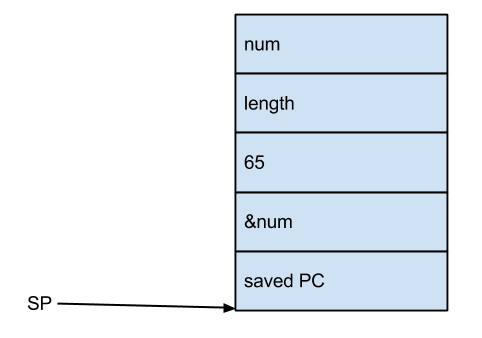
\includegraphics[scale = 0.4]{compile-error-code}\\
	\caption{编程范式 错误代码的编译}\label{fig.compile-error-code}
\end{figure}

在链接成功之后, 执行, 然后这是用到的就是真正的strlen, 发现参数只有一个, 而且参数的位置是
SP + 4, 也就是图中的 \&num 会被作为真正的参数

C++ 中函数可以重载, 而C 中不可以,
C 的汇编代码中, 函数的调用都是CALL 加上 函数名就够了
但是C++ 的汇编代码中, 函数的调用时CALL 加上 函数名而参数的类型列表. 之后这样才能区分重载函数的不同版本

\subsection{segmentation fault}
you dereference a bad pointer

例如对 NULL 指针 进行 * 运算
\begin{figure}[htbp]
	\centering
	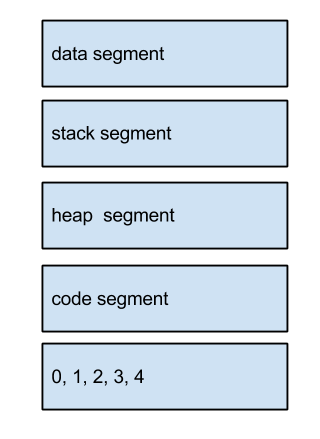
\includegraphics[scale = 0.4]{RAM}\\
	\caption{编程范式 RAM}\label{fig.RAM}
\end{figure}

地址0,1 2, 3, 4不在任何segment 中, 但是操作系统可以识别他们
所以当 * NULL, 也就是 * 0, 所以报 segmentation fault

\subsection{bus errors}
是对4 个段中的地址进行dereference, 但是这个地址并不是你认为可以引用的
\begin{lstlisting}[language = C]
void *vp=
*(short *)vp = 7;  //short 类型的地址不能以奇地址为首地址
*(int *)vp = 7;  //int类型只能以4 的倍数的整数地址为首地址, 所以 2002 就不行
\end{lstlisting}

\subsection{无线循环 缓冲区溢出}
\subsubsection{永真循环}
\begin{lstlisting}[language = C]
int main(){
int i;
int array[2];
for (i=0;i<=2;i++){
	array[i] = 0;
}
return 0;
}
\end{lstlisting}
\begin{figure}[htbp]
	\centering
	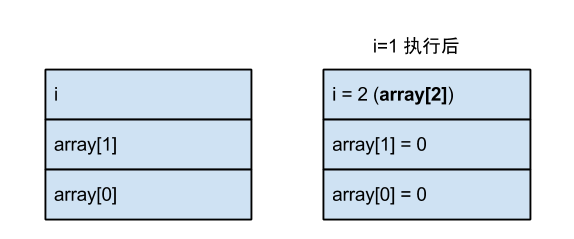
\includegraphics[scale = 0.4]{loop_forever}\\
	\caption{编程范式 永真循环}\label{fig.loop_forever}
\end{figure}

如图\ref{fig.编程范式.永真循环}中所示, i=1执行之后, i=2, 仍然满足循环条件, 所以继续执行array[2] = 0;\\
然后根据 array[2] 就是 SP+8, 也就是 i 的位置, 所以array[2] = 0;实际上是 i = 0; 然后发现又满足条件, 所以就会这样一直循环下去

\subsubsection{saved PC导致的无限循环}
\begin{lstlisting}[language = C]
void foo(){
int array[4];
int i;
for (i=0;i<=4;i++){
	arrar[i]  -= 4;
}
}
\end{lstlisting}
\begin{figure}[htbp]
	\centering
	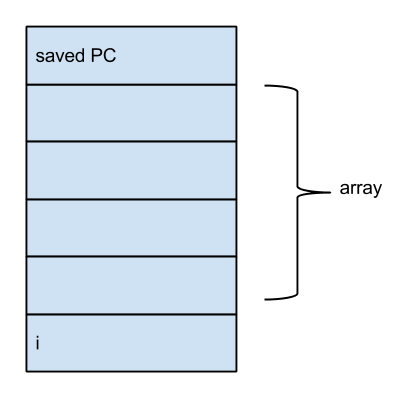
\includegraphics[scale = 0.4]{savedPC-loop}\\
	\caption{编程范式 savedPC导致的循环}\label{fig.savedPC-loop}
\end{figure}


在汇编代码中
CALL <foo>
instruction
在开始的时候foo 的activation record 中的saved PC保存的是指向 instruction 的地址
但是在foo执行的时候, 当i = 4 的时候, array[4] -= 4; 也就是将saved PC 的值减了4, 也就是有指向了 CALL <foo>, 这样当foo 执行完的时候, 又继续执行foo, 形成了一个无线循环

\section{Lecture 14}
\subsection{peseudo 全局变量}
\begin{lstlisting}[language = C]
int main(){
DeclareAndInitArray();
PrintArray();
}

void DeclareAndInitArray(){
int array[100];
int i;
for (i=0;i<100;i++){
	array[i] = i;
}
}

void PrintArray(){
int array[100];
int i;
for (i=0;i<100;i++){
	printf("%d\n",array[i]);
}
}
\end{lstlisting}
程序会输出结果, 而且看上去输出的就是DeclareAndInitArray 中赋的值, 但是这是由于在main 函数中, 执行DeclareAndInitArray 时, 申请的栈空间和执行PrintArray 申请的栈空间是一样的, 所以当行DeclareAndInitArray 执行完毕后, 栈指针SP 又回到了当初时的位置, 但是在行DeclareAndInitArray 中进行的数组赋值的内存内容并没有被清理(不会清理, 因为清理还需要消耗时间而且也没有这个必要), 所以行PrintArray 会输出之前的结果

printf\\
protype:	int printf(const char * control, ...);\\
返回值: 成功解析的占位符的个数

通过printf 的protype 我们可以解释\\
why we push parameters on the stack , why the $0$\textsuperscript{th} parameter is always at the bottom

\begin{lstlisting}[language = C]
printf("%d + %d = %d\n", 4, 5, 9);
\end{lstlisting}
\begin{figure}[htbp]
	\centering
	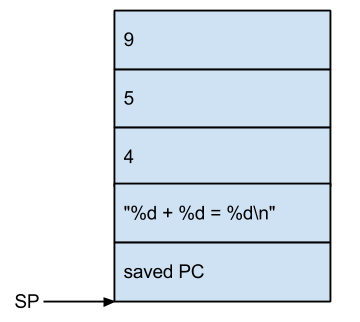
\includegraphics[scale = 0.4]{printf}\\
	\caption{编程范式 printf}\label{fig.printf}
\end{figure}

第0 个参数\verb "%d + %d = %d\n"是确定有的, 所以先输出, 当解析到 \%d 的时候, 知道上面肯定有额外的参数, 然后就进行替换; 然后一直进行下去 \\
因此第0 个参数, 也就是control 就像一个导航图,

PS: Pascal 中参数个数必须是确定的, 所以没有必要一定要 from right to left, 实际上Pascal 采用的是 from left to right

\section{Lecture 15 - multithreading}
\begin{lstlisting}[language = C]
int main(){
int numAgent = 10;
int numTicktes = 150;
InitThreadPackage(false);  // false表示不打印出线程的信息
for(int agent=0; agent <numAgents; agent++){
	char name[32];
	sprintf(name,"Agent %d Thread", agent);
	ThreadNew(name,SellTickets,2,agent, numTickets/numAgents); //name标记不同的线程
}
RunAllThreads();
return 0;
}

void SellTickets(int agentID, int numTicketToSell){
while (numTiketsToSell > 0){
	printf("Agent %d sells a ticket.\n", agentID);
	numTicketsToSell --;
	if(RandomChance(0.1))
ThreadSleep(1000);	 //0.1的概率 暂停1000毫秒
}
printf("Agent %d: All done.\n", agentID);
}
\end{lstlisting}
一个线程在执行SellTickets 的时候, 是可能被打断的, 然后处理器去执行其他的线程

C语言语句都不是atomic, 因为一个C语句会被翻译成好几个汇编语句

//让所有的agents 共享tickets
\begin{lstlisting}[language = C]
void SellTicktes(int agent, int *numTickets){
while( *numTickets > 0){
	(*numTickets) --;
}//critical region, 这while 循环应该是一个transaction, 不能让其他线程交叉进来
}

ThreadNew(name,SellTickets,2,agent, &numTickets);
\end{lstlisting}

\subsection{Semaphore - 信号量}
//形成一个transaction
\begin{lstlisting}[language = C]
int main(){
int numAgent = 10;
int numTicktes = 150;
Semaphore lock = SemaphoreNew(---, 1);  //第一个参数没有提到
InitThreadPackage(false);  // false表示不打印出线程的信息
for(int agent=0; agent <numAgents; agent++){
	char name[32];
	sprintf(name,"Agent %d Thread", agent);
	ThreadNew(name, SellTickets, 3, agent, &numTickets, lock);
}
RunAllThreads();
return 0;
}

void SellTickets(int agent, int *numTickets, Semaphore lock){
while(true){
	SemaphoreWait(lock);
if(*numTickets == 0 ) break; //如果为0, 立刻跳出循环并增加信号量
(*numTickets) --;
printf("....");
SemaphoreSignal(lock);
}
SemaphoreSignal(lock);
}
\end{lstlisting}

\textbf{Semaphore 信号量, 非负整数}
\begin{lstlisting}[language = C]
Semaphore lock = SemaphoreNew(---, 1);
\end{lstlisting}
//初始化为1,表示任一时刻, 只允许一个人进入critical region

\begin{lstlisting}[language = C]
SemaphoreWait(lock);  //减一操作 atomic --
SemaphoreSignal(lock); //加一操作 atomic ++
\end{lstlisting}
由于信号量不允许有非负整数变为负整数\\
当一个SemaphoreWait 发现一个 信号量为0 时, 他不会将其减为-1, 而是会等待, 并立即放弃处理器的控制权, 直到他检测到这个信号量被其他的进程作用SemaphoreSignal而变为正整数

如果我们当初将lock 初始化为0 的话, 因为已经到0 了, 不能再继续进行减一操作了, 所以所有的线程都会认为有某个线程占用这个lock, 导致所有的线程都在等待, 从而形成一个\textbf{死锁dead lock}

\section{Lecture 16}
考虑只有2 个agents 的情况
\begin{figure}[htbp]
	\centering
	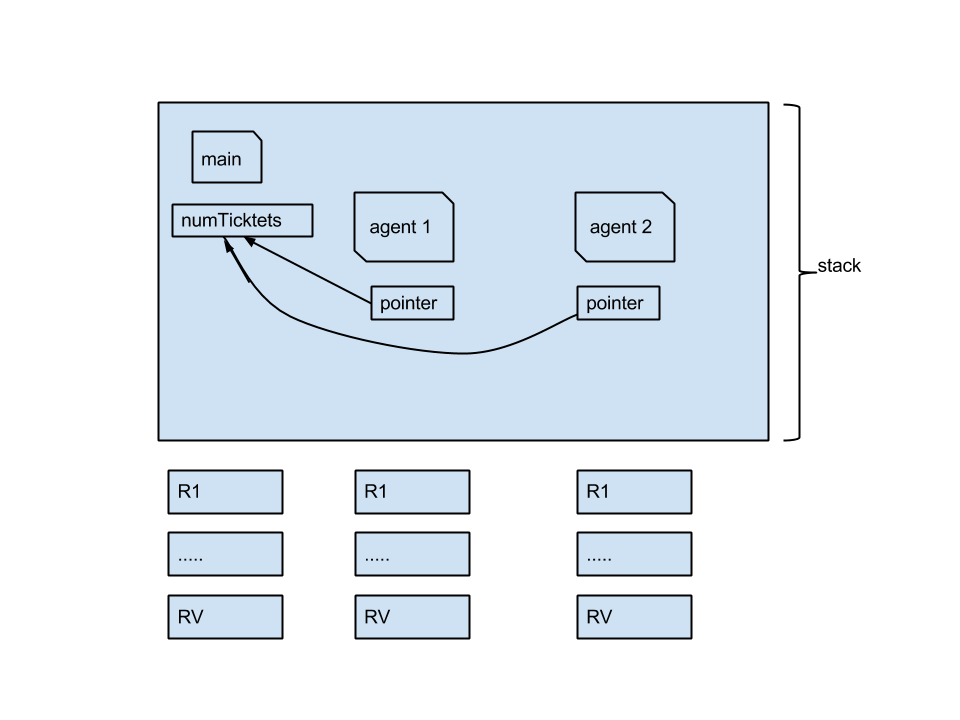
\includegraphics[scale = 0.4]{multi-thread_heap-stack}\\
	\caption{编程范式 多线程 堆栈}\label{fig.multi-thread.heap-stack}
\end{figure}

如图\ref{fig.编程范式.多线程.堆栈}中所示, 当一个线程被激活时, 他会获得进程的堆栈的副本, 然后这个线程运行, 然后运行之后, 再将线程的堆栈(共享信息)\\覆盖进程的堆栈中的共享信息, 因为在线程的运行过程中, 会对进行的共享信息进行修改, 所以必须同步到进程.\\
例如这里的情况, 当一个agent 售出一张票时, 他必须将进程的堆栈中的数据进行更新\\

\subsection{Writer and reader}
假设一台html server 与一个一台client browser
常见情况: 当一个页面加载到大概75\% 的时候, 你知道还有更多的内容. 表示服务器已经传递了75\% 的内容, 所以browser 的渲染过程必须被blocked, 以等待剩下的内容
下面的例子以上面的说明为指导性原则
我们使用8 个字符大小的缓冲区来模拟的服务器的填充缓冲区, client 从缓冲区读取数据

\begin{lstlisting}[language = C]
char buffer[8];
int main(){
InitThreadPackage(false);
ThreadNew("writer", writer, 0);
ThreadNew("reader", reader, 0);
RunAllThreads();
}

void writer(){
for (int i=0; i<40; i++){
	char c=PrepareRandomChar();
	buffer[i%8] = c;
}
}

void reader(){
for (int i=0; i<40; i++){
	char c= buffer[i%8] ;
	ProcessChar(c);
}
}
\end{lstlisting}
上面的程序的问题: writer 有可能严重超前于reader,导致有些数据还没有被reader 读取就已经被writer 重新覆盖掉了; 也有可能reader 严重超前于writer, 导致reader 读到了一些乱码, 因为这些位置还没有被writer 填充内容

解决办法: 信号量

\begin{lstlisting}[language = C]
char buffer[8];
Semaphore empty 8; //最开始, 剩余量是8, 表示可以write 8 个字符
Semaphore full 0; //最开始, 0, 表示可以read 0 个字符
int main(){
InitThreadPackage(false);
ThreadNew("writer", writer, 0);
ThreadNew("reader", reader, 0);
RunAllThreads();
}

void writer(){
for (int i=0; i<40; i++){
	char c=PrepareRandomChar(empty);
	SemaphoreWait(empty); //如果empty 可以继续减, 说明还有剩余空间供我们write
	buffer[i%8] = c;
SemaphoreSignal(full);
}
}

void reader(){
for (int i=0; i<40; i++){
	SemaphoreWait(full); // 如果full 可以继续减, 说明还有内容供我们read
	char c= buffer[i%8] ;
SemaphoreSignal(empty);
	ProcessChar(c);
}
}
\end{lstlisting}
这样最开始的时候 empty=8, 所以在没有reaer 插进来的情况下, writer 可以写8 次, 这时empty=0, 同时full=8, 当writer 想继续写的时候, 发现empty是0, 从而不能继续进行\\
而只有reader 才能对empty 进行增加的操作, 所以reader 可以执行, 同样, 在没有writer 插进来的情况下, reader 可以连续执行8 次. 这样就完成了一个轮回

如果最开始的时候, writer执行了1 次, empty=7, full=1; reader插进来了, full=1>0, 所以reader可以执行, 执行了1 次之后, empty=8, full=0, 回到了最开始的状态, 但是此时我们已经完成一个字符的写和读取

如果最开始的时候, reader 想执行, 但是发现full=0, 不能继续减下去, 所以只能由writer 先执行.

\subsection{哲学家与餐叉的故事- 死锁}
5 个哲学家
\begin{figure}[htbp]
	\centering
	
\includegraphics[scale = 0.4]{multi-thread_philo}\\
	\caption{编程范式 多线程 哲学家}\label{fig.multi-thread.philo}
\end{figure}

think, eat, think, eat, think, eat, go to bed;
\begin{lstlisting}[language = C]
Semaphore forks[]= {1, 1, 1, 1, 1}; //每个信号量表示了某项资源的可用性
void Philosopher(int id){
for(int i=0; i<3; i++){
	Think();
	SemaphoreWait(forks[id]);
	SemaphoreWait(forks[(id+1)%5]);
	Eat();
SemaphoreSignal(forks[id]);
	SemaphoreSignal(forks[(id+1)%5]);
}
}
\end{lstlisting}
在上面的这个函数中, 存在着一个dead lock 死锁的情形:\\
第1 个哲学家拿到了逆时针方向(右边)的餐叉; 这个时候, 处理器切换到了第2 个哲学家, 他也拿到了逆时针方向的餐叉, 依次下去, 所有人都拿到了逆时针方向的餐叉, 也就是说5 个人都拿到了餐叉. 在这个时候, 任何一个人想拿起第二把餐叉, 发现信号量为0, 于是所有人都失去处理器的控制权, 所有人都在等待左边人持有的某些资源. 这样就形成了一个死锁.
\textbf{所以当允许5 个人尝试去吃, 就可能形成死锁}

因为我们有5 个叉子, 所以任意时刻, 最多只有2 个人可以同时就餐\\
允许4 个尝试去吃
\begin{lstlisting}[language = C]
Semaphore forks[]= {1, 1, 1, 1, 1};
Semaphore numAllowedToEat = 4;
void Philosopher(int id){
for(int i=0; i<3; i++){
	Think();
SemaphoreWait(numAllowedToEat );
	SemaphoreWait(forks[id]);
	SemaphoreWait(forks[(id+1)%5]);
	Eat();
SemaphoreSignal(forks[id]);
	SemaphoreSignal(forks[(id+1)%5]);
SemaphoreSignal(numAllowedToEat );
}
}
\end{lstlisting}
这样, 当有4 个人尝试的时候, 可以将numAllowedToEat 由4 减为0, 当地5 个人尝试的时候就会失败, 所以这样我么就能保证只有4 个人可以尝试成功.

\section{Lecture 17}
numAllowedToEat 也可以被设置成2 或3, 但是设置成4 更好
That's the minimum amount of a fix that I need to implant into the code to make sure I do not have deadlock.
因为改动越小, 可以尽可能得留出足够多的弹性空间给线程管理器做规划

\subsection{FTP download}
简化版本的例子
\begin{lstlisting}[language = C]
int downloadSingleFile(const char *server, const char *path);
\end{lstlisting}
返回值: 下载的字节数

\begin{lstlisting}[language = C]
int downloadAllFiles(const char *server, const char *files[], int n){ // n files
int totalBytes = 0;
Semaphore lock = 1;
for (int i=0; i<n; i++){
	ThreadNew(-, downloadHelper, 4, server, files[i], totalBytes, lock);
}
return totalBytes;
}

void downloadHelper(const char *server, const char *path, int *numBytes, Semaphore lock){
int bytesDownloaded = downloadSingleFile(server, path);
SemaphoreWait(lock);
(*numBytes) += bytesDownloaded;
SemaphoreSignal(lock);
}


int downloadAllFiles(const char *server, const char *files[], int n){ // n files
Semaphore childDone = 0;
int totalBytes = 0;
Semaphore lock = 1;
for (int i=0; i<n; i++){
	ThreadNew(-, downloadHelper, 5, server, files[i], totalBytes, lock, childDone);
}
for (int i=0; i<n; i++){
	SemaphoreWait(childDone);
} // 等待所有线程完成下载任务, 然后才能return totalBytes
return totalBytes;
}

void downloadHelper(const char *server, const char *path, int *numBytes, Semaphore lock, Semaphore parentToSignal){
int bytesDownloaded = downloadSingleFile(server, path);
SemaphoreWait(lock);
(*numBytes) += bytesDownloaded;
SemaphoreSignal(lock);
SemaphoreSignal(parentToSignal);
}
\end{lstlisting}

\subsection{Ice cream store simulation}
manager, 检查冰淇淋是否合格\\
10 - 4- clerks, 制作冰淇淋  [10,40]\\
10 customers, 每个顾客会买, 随机1 到4 个冰淇淋\\
1 cashier

52 possible threads

\section{Lecture 18} important
\begin{lstlisting}[language = C]
int main(){
int totalCones=0;
InitThreadPackage();
SetupSemaphores();
for (int i=0; i< 10; i++){
	int numCones = RandomInteger(1,4);
	ThreadNew(, customer, 1, numCones);
	totalCones += numCones;
}
ThreadNew("cashier",cashier,0);
ThreadNew("manager", manager, 1, totalCones);
RunAllThreads();
FreeSemaphores();
return 0;
}

typedef struct {
bool passed;  // false in default
Semaphore requested; // initial to 0
Semaphore finished; // initial to 0
Semaphore lock; // initial to 1, 只允许一个人进入经理的办公室进行检查
}inspection;

void manager(int totalConesNeeded){
int numApproved = 0;
int numInspected = 0;
while (numApproved < totalConesNeeded){
	SW(inspection.requested); //SemaphoreWait
	numInspected ++;
	inspection.passed = RandomChoose(0,1);
	if(inspection.passed)
		numApproved ++;
	SS(inspection.finished);
}
}

void clerk(Semaphore semaTosignal){
bool passed = false;
while(!passed){
	makeCone();
	SW(inspection.lock);
	SS(inpection.requested); //如果为0, manager 将被阻塞, 只有clerk做完一个cone, 并且进入经理的办公室,但是这里有一个疑问, 既然已经进入了经理的办公室, 那说明里面没有其他的clerk, 应该说经理可以直接检查, 为什么还需要requeseted 这个信号量呢?
	SW(inspection.finished);
	passed = inspection.passed;
	SS(inspection.lock); //不管通过与否, 都要释放经理办公室的门锁
}
	SS(semaToSignal);
}

void customer(int numCones){
Semaphore clerksDone; // initial to 0
for(int i=0; i< numCones; i++){
	ThreadNew(, clerk, 1, clerksDone);	
}
for(int i=0; i< numCones; i++){
	SW(clerkDone);
}
SemaphoreFree(clerksDone);
WalkToCashier();
SW(line.lock);
int place = line.number ++;
SS(line.lock)
SS(line.requested);
SW(line.customers[place]);
}

typedef struct{
int number; // 0
Semaphore requested; //initial to 0
Semaphore customers[10]; //
Semaphore lock; // initial to 1对number的lock, 防止race condition
}line;

void cashier(){
for(int i=0; i<10, i++){
SW(line.requested);
checkout(i);
SS(line.customers[i];
}
}
\end{lstlisting}

\section{Lecture 19}
imperative: 因为主要是围绕动词展开的\\
procedural:
C

object-oriented:
C++

functional:
Scheme	runtime language

\begin{lstlisting}[language = Lisp]
(define Celsius→fahrenheit(temp)
	(+ 32 (* 1.8 temp)))
>(Celsius→fahreneit 100)  //shell
//212
\end{lstlisting}

\subsection{kawaa}
open source
\begin{verbatim}
>4
4
>"hello"
hello
>#f  //false
#f
>#t  //true
#t
>11.752
11.752
>11/5
11/5
>22/4
11/2
>(+ 1 2 3)  //递归求值
6
>(* (+ 4 4) (+ 5 5))
80
>(> 4 2)
#t
>(and (> 4 2) (< 10 5))
#f
\end{verbatim}

\bigskip\noindent
car 第一个元素 first  address register\\
cdr 余下的元素  data register\\
cons 合并\\
\begin{verbatim}
>(car '(1 2 3 4 5))  // 如果不用' ,那么第一个参数1 将被认为是一个函数
1
>(cdr '(1 2 3 4 5))
(2 3 4 5)
>>(car (cdr (cdr '(1 2 3 4 5))))
3
>(cdr '(4))
()
>(cdr '())
no
\end{verbatim}

\begin{lstlisting}[language = Lisp]
'(1 3 (4 (5)))
// 等价于
(quote (1 3 (4 (5))))  //就不计算他们的值, 只是按子读取
// ` 关闭quote
\end{lstlisting}

\begin{verbatim}
>(cons 1 '(2 3 4 5))  //第二个参数必须是列表
(1 2 3 4 5)
>(cons '(1 2 3) '(4 5))  //把第一个参数当做一个整体,加入到第二个参数(列表)中
((1 2 3) 4 5)

>(append '(1 2 3) '(4 5))
(1 2 3 4 5)
>(append '(1 2) '(3) '(4 5) '(6 7 8))
(1 2 3 4 5 6 7 8)

>(define add (x y)
	(+ x y))
ADD
>(add 10 7)
17
>(add "Hi" "there")
error

>(sum-of '(1 2 3 4))
\end{verbatim}

sum-of的实现方式, 不使用Scheme 默认的迭代方式
\begin{lstlisting}[language = Lisp]
(define sum-of (numlist)
	(if (null? numlist) 0
		(+ (car numlist) (sum-of (cdr numlist))))) //otherwise
\end{lstlisting}

\section{Lecture 20}
\begin{verbatim}
>(num-of '("hello" 1 2 3 4 5))
\end{verbatim}
只有当要计算(+ "hello" 15)的时候才能发现这个错误

\begin{lstlisting}[language = Lisp]
(define fib (n)
	if (zero? n) 0
		(if (= n 1) 1
			(+ (fib (- n 1))
				(fib (- n 2)))))

(define fib (n)
	if (or (= n 0)
			(= n 1)) n
		(+ (fib (- n 1))
			(fib (- n 2))))
\end{lstlisting}

\begin{verbatim}
>(if (zero? 0) 4
	 (+ "hello" 4.5 '(8 2)))
4
// 由于Scheme 是runtime language, 所以仍然能够运行, 而不会像C等编译型语言那样对"hello"+4.5 在编译阶段报错

>(flatten '(1 2 3 4))
(1 2 3 4)
>(flatten '(1 (2 "3") 4 ((5))))
(1 2 "3" 4 5)
>(flatten '(1 2 () 3 4))
(1 2 3 4)
\end{verbatim}

实现flatten 函数需要考虑的三种情况
\begin{enumerate}
	\item '()
	\item '(1 elements)
	\item '((1 2) elements)
\end{enumerate}

\begin{lstlisting}[language = Lisp]
(define flatten (sequence)
	(cond (((null? sequence) '())
			((list? (car sequence)
				(append (flatten (car sequence))
						(flatten (cdr sequence)))
			(else (cons (car sequence) (flatten (cdr sequence))))))))

(define sorted? (num-list)
	(or (< (length num-list) 2)
		(and (<= (car num-list) (cadr num-list))
			(sorted? (cdr num-list)))))
\end{lstlisting}

\bigskip\noindent
cadr: (cadr list) == (car (cdr list))\\
cddddr\\
cadadr\\
c 和r 之间最多有4个

\begin{verbatim}
>(sorted '(1 2 2 4 7))
#t
>(sorted '(1 0 4 7 10))
#f
>(<= 1 2 3 4 5 6 6)
#t   //但是不推荐这种用法
\end{verbatim}

\subsection{内存模型}
\begin{lstlisting}[language = Lisp]
(car '(1 2 3 4))
\end{lstlisting}
\begin{figure}[htbp]
	\centering
	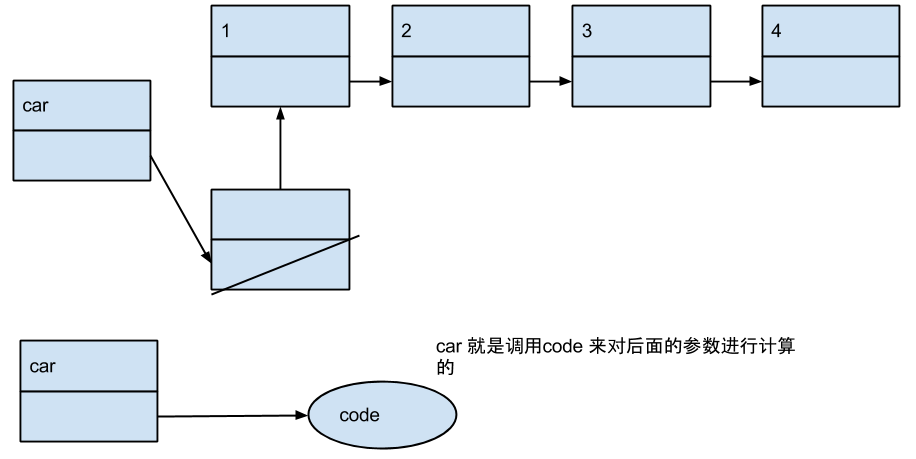
\includegraphics[scale = 0.4]{scheme_memo_model}\\
	\caption{Scheme 内存模型}\label{fig.scheme.memo.model}
\end{figure}


\begin{verbatim}
>(sorted? '(1 2 3 4) <=)
#t
>(sorted? '("a" "b" "c" "d") string<?)
#t
\end{verbatim}
定义如下
\begin{lstlisting}[language = Lisp]
(define sorted? (seq comp)
	(or (< (length seq) 2)
		(and (comp (car seq) (cadr seq))
			(sorted? (cdr seq) comp))))
\end{lstlisting}

\section{Lecture 21}
.scm file
\begin{verbatim}
>load "test.scm"  //然后就可以调用test.scm 中定义的函数

>(double-all '(1 2 3 4))
(2 4 6 8)
>(increment-all '(1 2 3 4))
(2 3 4 5)

(define double x (* x 2))
(define incr x (+ x 1))

>(map double '(1 2 3 4))  //对每个元素进行double 运算
(2 4 6 8)
>(map incr '(1 2 3 4))
(2 3 4 5)
>(map cons '(1 2 8) '((4) () (2 5)))
((1 4) (2) (8 2 5))
>(map + '(1 2) '(3 4) '(6 10))
(10 16)
>(map + '(1 2) '(3 4 1) '(6 10)) //在最小的列表结束后, 运算就结束了, 其他列表多余的元素会被忽略
(10 16)
\end{verbatim}

\begin{lstlisting}[language = Lisp]
(define (my-unary-map fn seq)
	(if (null? seq) '()
		(cons (fn (car seq)) (my-unary-map fn (cdr seq)))))
\end{lstlisting}

\subsection{apply}
\begin{verbatim}
>(apply + '(1 2 3))
6
\end{verbatim}apply 不能用在and, or 等非真正的函数上面

\begin{lstlisting}[language = Lisp]
(define (average num-list)
	(/ (apply + num-list) (length num-list)))

(define (flatten seq)
	(if (not (list? seq) (list seq)
	(apply append (map flatten seq)))))
\end{lstlisting}

\begin{verbatim}
>(flatten ((1 2) ((3) ((4) 5)) 10))
(1 2 3 4 5 10)
(append append ((flatten (1 2)) (flatten ((3) ((4) 5))) (flatten 10)))
(flatten (1 2)) == (apply append ((flatten 1) (flatten 2))) == (apply append ((1) (2))) == (1 2) //推断是生成这样的, 但是((flatten 1) (flatten 2))==(((1) (2))) 括号的深度好像有问题
\end{verbatim}

\subsection{eval}
\begin{verbatim}
>'(+ 1 2 3) //抑制evaluation
(+ 1 2 3)
>(eval '(+ 1 2 3))  //强制进行evaluation
6
\end{verbatim}

\begin{lstlisting}[language = Lisp]
(define (translate points delta)
	(map (lambda (x) (+ x delta)) points)
)

(define (translate seq delta)
	(define shift-by x) (+ x delta)
	(map shift-by seq))
\end{lstlisting}

\begin{verbatim}
>(translate '(2 5 8 11 25) 100)
(102 105 108 111 125)
\end{verbatim}

\begin{lstlisting}[language = Lisp]
(define (sum x y) (+ x y))
(define sum (lambda (x y) (+ x y))) //sum 被绑定到这个匿名函数上
(define PI 3.14)
\end{lstlisting}

\section{Lecture 22}
power set: a set which contains all of its subsets
\begin{verbatim}
(1 2 3)的子集
(() (2) (3) (2 3)
(1) (1 2) (1 3) (1 2 3))
第二行相当于: cons 1 with (() (2) (3) (2 3))

>(power-set '())
(())
\end{verbatim}

\begin{lstlisting}[language = Lisp]
(define (ps set)
	(if (null? set) '(())
		(append (ps (cdr set))
			(map (lambda (subset) (cons (car set) subset)) (ps (cdr set)))
		)
	)
)

(ps (cdr set)) // 重复调用

(define (ps set)
	(if (null? set) '(())
		(let ((ps-rest (ps (cdr set))))
			(append ps-rest
				(map (lambda (subset) (cons (car set) subset))
					ps-rest
				)
			)
		)
	)
)

(let ((x exp1)
	(y exp2)
	(z exp3))
//using x y z
)

(let ((x -)
	(y -))
(a x y)
)
//相当于
((lambda (x y) (a x y)) - -)
\end{lstlisting}

\begin{verbatim}
>(permute '(1 2 3))
((1 2 3) (1 3 2)
 (2 1 3) (2 3 1)
 (3 1 2) (3 2 1))
>(permute '(1 2 3 4))
\end{verbatim}
\begin{figure}[htbp]
	\centering
	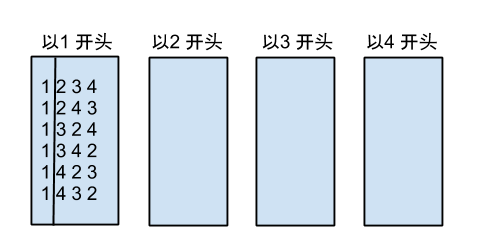
\includegraphics[scale = 0.4]{scheme_permute}\\
	\caption{scheme permute}\label{fig.scheme.permute}
\end{figure}

在第一个方框中, 我们可以看到以1 开头的排列后面刚好是 2 3 4 的全排列

\todo{个函数没有看懂}
\begin{lstlisting}[language = Lisp]
(define (permute items)
	(apply append
		(map (lambda (elem)
			(map (lambda (permutation) (cons elem permutation))
			(permute (remove items elem)))))
		items))
\end{lstlisting}

\textbf{All lists are immutable}

self-type identifying
\begin{verbatim}
>4  //Scheme 解释器将你输入的4 解释为整数(define (ps set)
\end{verbatim}
在第一个方框中, 我们可以看到以1 开头的排列后面刚好是 2 3 4 的全排列

\begin{verbatim}
>'(1 2 3)
//等价于:
(cons 1 (cons 2 (cons 3 '())))
//对于第一个元素来说, 1 是car field, 后面的(cons 2 (cons 3 '()))是 cdr field
\end{verbatim}
\begin{figure}[htbp]
	\centering
	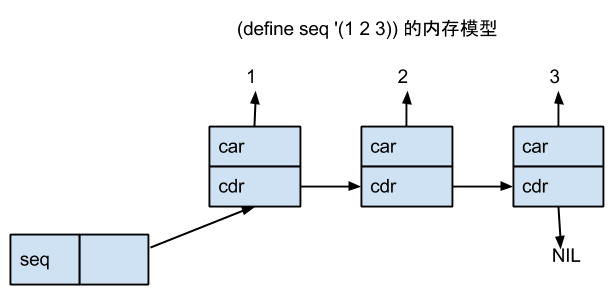
\includegraphics[scale = 0.4]{scheme_memo_model2}\\
	\caption{scheme 内存模型2}\label{fig.scheme.memo.model2}
\end{figure}

\section{Lecture 23}
当我们请求
\begin{verbatim}
>(car seq)   // 找到第一个car, 也就是图中的1所在的car
1
>(cdr seq)
(2 3)
>(cons '(1 2 3) '(4 5 6))
((1 2 3) 4 5 6)
\end{verbatim}
\begin{figure}[htbp]
	\centering
	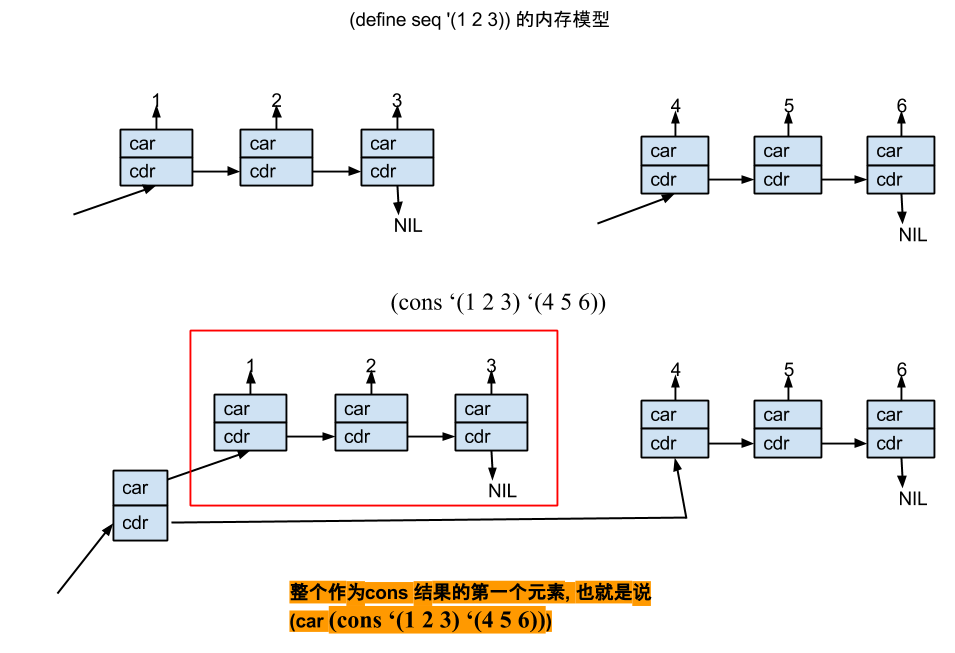
\includegraphics[scale = 0.4]{scheme_cons}\\
	\caption{scheme cons}\label{fig.scheme.cons}
\end{figure}

从12:00 minutes 继续看

\section{Lecture 24}
Python:
scripting language,
imperative,
object-oriented,
functional.

\begin{verbatim}
?> x = 5  //这个地方实际上输出的是None, 但是由于None 是不可见的, 所以我们看不到任何输出, None 有点类似于C 中的void
?>x
5
?>"Iron Man".istitle()
True
?>"hello there".istitle()
False
\end{verbatim}

\section{Lecture 25}
\begin{verbatim}
>>>
>>> a = [10, 12, 14]
>>> a
[10, 12, 14]
>>> w = [a,a]
>>> w
[[10, 12, 14] [10, 12, 14]]
>>> a.append(17)
>>> a
[10, 12, 14, 17]
>>> w
[[10, 12, 14, 17] [10, 12, 14, 17]]
\end{verbatim}
默认的几乎都是浅拷贝, 也就是只是把地址拷贝过去用, 而不是把地址所指向的内容全部拷贝过去

\begin{verbatim}
from copy import copy,deepcopy
copy 只拷贝一层, 所以当有一个list of list时, 第二层和原来的还是共享内存的
deepcopy 完全的拷贝
testcopy.py
\end{verbatim}

\begin{lstlisting}[language = Python]
#-*- coding:utf-8 -*-
 from copy import copy, deepcopy
 x=[1,2,[4,5]]
 print "orignal x: ",x
 y=copy(x)
 z=deepcopy(x)
 t=x
 print "y is x: ",y is x
 print "z is x: ",z is x
 print "t is x: ",t is x
 print "list in list x: ",x[2]
 x[2].append(10)
 x.append(6)
 print "after appending, current x: ",x
 print "copy: ",y
 print "deepcopy: ",z
 print "t=x, t: ",t
 \end{lstlisting}
\begin{figure}[htbp]
	\centering
	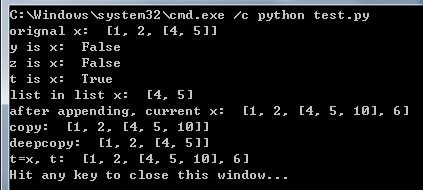
\includegraphics[scale = 0.7]{copy_deep}\\
	\caption{Deep copy}\label{fig.copy.deep}
\end{figure}

\section{Lecture 26}
xml

\begin{lstlisting}[language = Python]
#-*- coding:utf-8 -*-
from urllib2 import urlopen
from xml.sax import make.parser, ContentHandler
import sys
\end{lstlisting}

\section{Lecture 27}
\subsection{Haskell}
Functional
\begin{enumerate}
	\item Lisp/Scheme (1959)
	\item ML/OCamml (1979)
	\item Miranda (1985)
	\item Haskell 98 (1959)
\end{enumerate}
Haskell is neat
Haskell 中的列表中所有元素必须是相同类型的
\begin{verbatim}
map (+ 1) [3, 2, 5] => [4, 3, 6]
\end{verbatim}

Fibonacci
\begin{verbatim}
fib = 1:1:zipWith (+) fib (tail fib)
\end{verbatim}

\bigskip\noindent
1:1 前两个元素\\
zipWith is like a map function

\begin{verbatim}
if a then b else c
\end{verbatim}

\bigskip\noindent
Types:integer, float, char\\
Like Scheme, functions are a type

User types
\begin{verbatim}
data Bool = True | False
\end{verbatim}
\end{document}
